\documentclass{ximera}


\graphicspath{
  {./}
  {ximeraTutorial/}
  {basicPhilosophy/}
}

\newcommand{\mooculus}{\textsf{\textbf{MOOC}\textnormal{\textsf{ULUS}}}}

\usepackage{tkz-euclide}\usepackage{tikz}
\usepackage{tikz-cd}
\usetikzlibrary{arrows}
\tikzset{>=stealth,commutative diagrams/.cd,
  arrow style=tikz,diagrams={>=stealth}} %% cool arrow head
\tikzset{shorten <>/.style={ shorten >=#1, shorten <=#1 } } %% allows shorter vectors

\usetikzlibrary{backgrounds} %% for boxes around graphs
\usetikzlibrary{shapes,positioning}  %% Clouds and stars
\usetikzlibrary{matrix} %% for matrix
\usepgfplotslibrary{polar} %% for polar plots
\usepgfplotslibrary{fillbetween} %% to shade area between curves in TikZ
\usetkzobj{all}
\usepackage[makeroom]{cancel} %% for strike outs
%\usepackage{mathtools} %% for pretty underbrace % Breaks Ximera
%\usepackage{multicol}
\usepackage{pgffor} %% required for integral for loops



%% http://tex.stackexchange.com/questions/66490/drawing-a-tikz-arc-specifying-the-center
%% Draws beach ball
\tikzset{pics/carc/.style args={#1:#2:#3}{code={\draw[pic actions] (#1:#3) arc(#1:#2:#3);}}}



\usepackage{array}
\setlength{\extrarowheight}{+.1cm}
\newdimen\digitwidth
\settowidth\digitwidth{9}
\def\divrule#1#2{
\noalign{\moveright#1\digitwidth
\vbox{\hrule width#2\digitwidth}}}






\DeclareMathOperator{\arccot}{arccot}
\DeclareMathOperator{\arcsec}{arcsec}
\DeclareMathOperator{\arccsc}{arccsc}

















%%This is to help with formatting on future title pages.
\newenvironment{sectionOutcomes}{}{}



\outcome{Compute dot products.}
\outcome{Use dot products to compute the angle between vectors.}
\outcome{Find orthogonal projections.}
\outcome{Use the dot product in applied settings.}

\title[Dig-In:]{The dot product}

\begin{document}
\begin{abstract}
  The dot product measures how aligned two vectors are with each
  other.
\end{abstract}
\maketitle


\section{The definition of the dot product}

We have already seen how to add vectors and how to multiply vectors by
scalars.

\begin{warning}
We have not yet defined how to multiply a vector by a vector.  You
might think it is reasonable to define
\[
\begin{bmatrix}
  a_1\\
  a_2\\
  \vdots\\
  a_n
\end{bmatrix}
\cdot
\begin{bmatrix}
  b_1\\
  b_2\\
  \vdots\\
  b_n
\end{bmatrix}
=
\begin{bmatrix}
  a_1b_1\\
  a_2b_2\\
  \vdots\\
  a_nb_n
\end{bmatrix}
\] 
but this operation is not especially useful, and will \textbf{never be
  utilized in this course}.
\end{warning}

In this section we will define a way to ``multiply'' two vectors
called the \textit{dot product}. The dot product measures how
``aligned'' two vectors are with each other.

\begin{definition}
  The \textbf{dot product} of two vectors is given by the following.
  \begin{align*}
  \begin{bmatrix}
    a_1\\
    a_2\\
    \vdots\\
    a_n
  \end{bmatrix}
  \bullet
  \begin{bmatrix}
    b_1\\
    b_2\\
    \vdots\\
    b_n
  \end{bmatrix}
  &= \sum_{i=1}^n a_ib_i\\
  &= a_1b_1 + a_2b_2 +\dots+a_nb_n
  \end{align*}
\end{definition}

The first thing you should notice about the the dot product is that
\[
\mathbf{vector}\bullet \mathbf{vector} = \mathbf{number}.
\]
\begin{question}
  Compute.
  \[
  \left\langle 1,2,3 \right\rangle \bullet \left\langle 4,5,6 \right\rangle
  \begin{prompt}
    = \answer{32}
  \end{prompt}
  \]
  \begin{question}
  Compute.
  \[
  \left\langle 1,1,-1 \right\rangle \bullet \left\langle 1,1,2 \right\rangle
  \begin{prompt}
    = \answer{0}
  \end{prompt}
  \]
\end{question}
\end{question}

\begin{question}
  Let $\overset{\boldsymbol{\rightharpoonup}}{\mathbf{u}},\overset{\boldsymbol{\rightharpoonup}}{\mathbf{v}},\overset{\boldsymbol{\rightharpoonup}}{\mathbf{w}}$ be nonzero vectors in $\mathbb{R}^3$. Which of
  the following expressions make sense?
  \begin{selectAll}
    \choice[correct]{$(\overset{\boldsymbol{\rightharpoonup}}{\mathbf{w}} \bullet \overset{\boldsymbol{\rightharpoonup}}{\mathbf{u}} ) \overset{\boldsymbol{\rightharpoonup}}{\mathbf{u}}$}
    \choice[correct]{$5(\overset{\boldsymbol{\rightharpoonup}}{\mathbf{u}} +\overset{\boldsymbol{\rightharpoonup}}{\mathbf{w}}) \bullet {\overset{\boldsymbol{\rightharpoonup}}{\mathbf{u}}}$}
    \choice{$\overset{\boldsymbol{\rightharpoonup}}{\mathbf{w}} / \overset{\boldsymbol{\rightharpoonup}}{\mathbf{u}}$}
    \choice[correct]{$\left\langle 2,3 \right\rangle \bullet \left\langle 4,2 \right\rangle + 7$}
    \choice[correct]{$\overset{\boldsymbol{\rightharpoonup}}{\mathbf{w}} / ( \overset{\boldsymbol{\rightharpoonup}}{\mathbf{u}} \bullet \overset{\boldsymbol{\rightharpoonup}}{\mathbf{u}})$}
    \choice{$\left\langle 1,3 \right\rangle \bullet \left\langle -1,2,5 \right\rangle$}
    \choice{$\overset{\boldsymbol{\rightharpoonup}}{\mathbf{u}}\bullet \overset{\boldsymbol{\rightharpoonup}}{\mathbf{v}}+\overset{\boldsymbol{\rightharpoonup}}{\mathbf{w}}$}
  \end{selectAll}
  \begin{hint}
    Think about which terms/factors are vectors and which
    terms/factors are scalars.
  \end{hint}
  \begin{question}
    Which of the following are vectors?
    \begin{selectAll}
    \choice[correct]{$(\overset{\boldsymbol{\rightharpoonup}}{\mathbf{w}} \bullet \overset{\boldsymbol{\rightharpoonup}}{\mathbf{u}} ) \overset{\boldsymbol{\rightharpoonup}}{\mathbf{u}}$}
    \choice{$5(\overset{\boldsymbol{\rightharpoonup}}{\mathbf{u}} +\overset{\boldsymbol{\rightharpoonup}}{\mathbf{w}}) \bullet {\overset{\boldsymbol{\rightharpoonup}}{\mathbf{u}}}$}
    \choice{$\left\langle 2,3 \right\rangle \bullet \left\langle 4,2 \right\rangle + 7$}
    \choice[correct]{$\overset{\boldsymbol{\rightharpoonup}}{\mathbf{w}} / ( \overset{\boldsymbol{\rightharpoonup}}{\mathbf{u}} \bullet \overset{\boldsymbol{\rightharpoonup}}{\mathbf{u}})$}
    \end{selectAll}
  \end{question}
\end{question}

The dot product allows us to write some complicated formulas more simply.

\begin{theorem}
  The magnitude of vector $\overset{\boldsymbol{\rightharpoonup}}{\mathbf{v}}$ is given by
  \[
  |\overset{\boldsymbol{\rightharpoonup}}{\mathbf{v}}|=\sqrt{\overset{\boldsymbol{\rightharpoonup}}{\mathbf{v}}\bullet\overset{\boldsymbol{\rightharpoonup}}{\mathbf{v}}}
  \]
  \begin{explanation}
    We already know that if $\overset{\boldsymbol{\rightharpoonup}}{\mathbf{v}} = \left\langle v_1,v_2,\dots,v_n \right\rangle$,
    then
    \[
    |\overset{\boldsymbol{\rightharpoonup}}{\mathbf{v}}| = \sqrt{v_1^2+v_2^2+v_3^2+\dots+v_n^2}
    \]
    but
    \[
    \overset{\boldsymbol{\rightharpoonup}}{\mathbf{v}} \bullet \overset{\boldsymbol{\rightharpoonup}}{\mathbf{v}} = v_1^2+v_2^2+v_3^2+\dots+v_n^2,
    \]
    so
    \[
    |\overset{\boldsymbol{\rightharpoonup}}{\mathbf{v}}|=\sqrt{\overset{\boldsymbol{\rightharpoonup}}{\mathbf{v}}\bullet\overset{\boldsymbol{\rightharpoonup}}{\mathbf{v}}}.
    \]
  \end{explanation}
\end{theorem}

\begin{question}
  Compute the magnitude of the vector $\overset{\boldsymbol{\rightharpoonup}}{\mathbf{v}} = \left\langle 1,2,3,4 \right\rangle$.
  \begin{prompt}
    \[
    |\overset{\boldsymbol{\rightharpoonup}}{\mathbf{v}}| = \answer{\sqrt{30}}
    \]
  \end{prompt}
\end{question}








\section{The geometry of the dot product}

Let's see if we can figure out what the dot product tells us geometrically. As
an appetizer, we give the next theorem: the Law of Cosines.

\begin{theorem}[Law of Cosines]
  Given a triangle with sides of length $a$, $b$, and $c$, and with
  $0\le\theta\le\pi$ being the measure of the angle between the sides
  of length $a$ and $b$,
  \begin{image}
    \begin{tikzpicture}
    \draw (.5,.1) arc[radius=.5cm,start angle=11.3,end angle=56.3];
    \draw[ultra thick,penColor] (0,0) -- (5,1) -- (2,3)--(0,0)--cycle;
    \node[below,penColor] at (2.5,.5) {$a$}; %% <a,b>
    \node[above left,penColor] at (1,1.5) {$b$}; %% <c,d>
    \node[above right,penColor] at (3.5,2) {$c$}; %% <c,d>
    \node[above right] at (.4,.2) {$\theta$}; %% <c,d>
\end{tikzpicture}
  \end{image}
  we have
  \[
  c^2 = a^2+b^2-2ab\cos(\theta).
  \]
\end{theorem}
\begin{question}
  When $\theta = \pi/2$ what does the law of cosines say?
  \begin{prompt}
    \begin{multipleChoice}
      \choice[correct]{It is the Pythagorean theorem.}
      \choice{It is the law of sines.}
      \choice{It is undefined.}
    \end{multipleChoice}
  \end{prompt}
\end{question}

We can rephrase the Law of Cosines in the language of vectors.  The
vectors $\overset{\boldsymbol{\rightharpoonup}}{\mathbf{v}}$, $\overset{\boldsymbol{\rightharpoonup}}{\mathbf{w}}$, and $\overset{\boldsymbol{\rightharpoonup}}{\mathbf{v}} - \overset{\boldsymbol{\rightharpoonup}}{\mathbf{w}}$ form a triangle
\begin{image}
  \begin{tikzpicture}
    \draw (.5,.1) arc[radius=.5cm,start angle=11.3,end angle=56.3];
    \draw[->,ultra thick,penColor] (0,0) -- (5,1);
    \draw[->,ultra thick,penColor2] (0,0) -- (2,3);
    \draw[->,ultra thick,penColor3] (2,3) -- (5,1);
    \node[below,penColor] at (2.5,.5) {$\overset{\boldsymbol{\rightharpoonup}}{\mathbf{v}}$}; %% <a,b>
    \node[above left,penColor2] at (1,1.5) {$\overset{\boldsymbol{\rightharpoonup}}{\mathbf{w}}$}; %% <c,d>
    \node[above right,penColor3] at (3.5,2) {$\overset{\boldsymbol{\rightharpoonup}}{\mathbf{v}}-\overset{\boldsymbol{\rightharpoonup}}{\mathbf{w}}$}; %% <c,d>
    \node[above right] at (.4,.2) {$\theta$}; %% <c,d>
\end{tikzpicture}
\end{image}
so if $\theta$ is the angle between $\overset{\boldsymbol{\rightharpoonup}}{\mathbf{v}}$ and $\overset{\boldsymbol{\rightharpoonup}}{\mathbf{w}}$ we must
have
\[
|\overset{\boldsymbol{\rightharpoonup}}{\mathbf{v}} - \overset{\boldsymbol{\rightharpoonup}}{\mathbf{w}}|^2=|\overset{\boldsymbol{\rightharpoonup}}{\mathbf{v}}|^2+|\overset{\boldsymbol{\rightharpoonup}}{\mathbf{w}}|^2-2|\overset{\boldsymbol{\rightharpoonup}}{\mathbf{w}}||\overset{\boldsymbol{\rightharpoonup}}{\mathbf{v}}|\cos(\theta).
\]



\begin{theorem}[Geometric Interpretation of the Dot Product]\index{dot product}
  For any two vectors $\overset{\boldsymbol{\rightharpoonup}}{\mathbf{v}}$ and $\overset{\boldsymbol{\rightharpoonup}}{\mathbf{w}}$,
  \[
  \overset{\boldsymbol{\rightharpoonup}}{\mathbf{v}} \bullet \overset{\boldsymbol{\rightharpoonup}}{\mathbf{w}} = |\overset{\boldsymbol{\rightharpoonup}}{\mathbf{v}}||\overset{\boldsymbol{\rightharpoonup}}{\mathbf{w}}|\cos(\theta)
  \]
  where $0\le \theta\le\pi$ is the angle between $\overset{\boldsymbol{\rightharpoonup}}{\mathbf{v}}$ and
  $\overset{\boldsymbol{\rightharpoonup}}{\mathbf{w}}$.
  \begin{explanation}
    First note that
    \[
    |\overset{\boldsymbol{\rightharpoonup}}{\mathbf{v}} - \overset{\boldsymbol{\rightharpoonup}}{\mathbf{w}}|^2 =  (\overset{\boldsymbol{\rightharpoonup}}{\mathbf{v}} - \overset{\boldsymbol{\rightharpoonup}}{\mathbf{w}})\bullet(\overset{\boldsymbol{\rightharpoonup}}{\mathbf{v}} - \overset{\boldsymbol{\rightharpoonup}}{\mathbf{w}})
    \]
    Now use the law of cosines to write
    \begin{align*}
      |\overset{\boldsymbol{\rightharpoonup}}{\mathbf{v}} - \overset{\boldsymbol{\rightharpoonup}}{\mathbf{w}}|^2&=|\overset{\boldsymbol{\rightharpoonup}}{\mathbf{v}}|^2+|\overset{\boldsymbol{\rightharpoonup}}{\mathbf{w}}|^2-2|\overset{\boldsymbol{\rightharpoonup}}{\mathbf{v}}||\overset{\boldsymbol{\rightharpoonup}}{\mathbf{w}}|\cos(\theta)\\
      (\overset{\boldsymbol{\rightharpoonup}}{\mathbf{v}} - \overset{\boldsymbol{\rightharpoonup}}{\mathbf{w}})\bullet(\overset{\boldsymbol{\rightharpoonup}}{\mathbf{v}} - \overset{\boldsymbol{\rightharpoonup}}{\mathbf{w}}) &=|\overset{\boldsymbol{\rightharpoonup}}{\mathbf{v}}|^2+|\overset{\boldsymbol{\rightharpoonup}}{\mathbf{w}}|^2-2|\overset{\boldsymbol{\rightharpoonup}}{\mathbf{v}}||\overset{\boldsymbol{\rightharpoonup}}{\mathbf{w}}|\cos(\theta)\\
      \overset{\boldsymbol{\rightharpoonup}}{\mathbf{v}}\bullet\overset{\boldsymbol{\rightharpoonup}}{\mathbf{v}} -2\overset{\boldsymbol{\rightharpoonup}}{\mathbf{v}}\bullet\overset{\boldsymbol{\rightharpoonup}}{\mathbf{w}}+\overset{\boldsymbol{\rightharpoonup}}{\mathbf{w}}\bullet\overset{\boldsymbol{\rightharpoonup}}{\mathbf{w}}&=|\overset{\boldsymbol{\rightharpoonup}}{\mathbf{v}}|^2+|\overset{\boldsymbol{\rightharpoonup}}{\mathbf{w}}|^2-2|\overset{\boldsymbol{\rightharpoonup}}{\mathbf{v}}||\overset{\boldsymbol{\rightharpoonup}}{\mathbf{w}}|\cos(\theta)\\
      |\overset{\boldsymbol{\rightharpoonup}}{\mathbf{v}}|^2+|\overset{\boldsymbol{\rightharpoonup}}{\mathbf{w}}|^2 -2\overset{\boldsymbol{\rightharpoonup}}{\mathbf{v}}\bullet\overset{\boldsymbol{\rightharpoonup}}{\mathbf{w}} &=|\overset{\boldsymbol{\rightharpoonup}}{\mathbf{v}}|^2+|\overset{\boldsymbol{\rightharpoonup}}{\mathbf{w}}|^2-2|\overset{\boldsymbol{\rightharpoonup}}{\mathbf{v}}||\overset{\boldsymbol{\rightharpoonup}}{\mathbf{w}}|\cos(\theta)\\
      \overset{\boldsymbol{\rightharpoonup}}{\mathbf{v}} \bullet \overset{\boldsymbol{\rightharpoonup}}{\mathbf{w}} &= |\overset{\boldsymbol{\rightharpoonup}}{\mathbf{v}}||\overset{\boldsymbol{\rightharpoonup}}{\mathbf{w}}|\cos(\theta).
    \end{align*}
  \end{explanation}
\end{theorem}

The theorem above tells us some interesting things about the angle 
between two (nonzero) vectors.

\begin{theorem}
  If $\overset{\boldsymbol{\rightharpoonup}}{\mathbf{v}}$ and $\overset{\boldsymbol{\rightharpoonup}}{\mathbf{w}}$ are two nonzero vectors, and $\theta$ is
  the angle between them,
  \[
  \overset{\boldsymbol{\rightharpoonup}}{\mathbf{v}}\bullet \overset{\boldsymbol{\rightharpoonup}}{\mathbf{w}} = 0 \text{ if and only if } \theta=
  \frac{\pi}{2}.
  \]
\end{theorem}

We have a special buzz-word for when the dot product is zero.

\begin{definition}
  Two vectors are called \textbf{orthogonal} if the the dot product of
  these vectors is zero. Geometrically, this means that the angle
  between the vectors is $\pi/2$ or $90^\circ$. Note, this also means
  that the zero vector is orthogonal to all vectors.
\end{definition}

From this we see that the dot product of two vectors is zero if those
vectors are orthogonal.  Moreover, if the dot product is not zero,
using the formula
\[
\overset{\boldsymbol{\rightharpoonup}}{\mathbf{v}} \bullet \overset{\boldsymbol{\rightharpoonup}}{\mathbf{w}} = |\overset{\boldsymbol{\rightharpoonup}}{\mathbf{v}}||\overset{\boldsymbol{\rightharpoonup}}{\mathbf{w}}|\cos(\theta)
\]
allows us to compute the angle between these vectors via
\[
\theta = \arccos\left(\frac{\overset{\boldsymbol{\rightharpoonup}}{\mathbf{v}} \bullet \overset{\boldsymbol{\rightharpoonup}}{\mathbf{w}}
}{|\overset{\boldsymbol{\rightharpoonup}}{\mathbf{v}}|\cdot|\overset{\boldsymbol{\rightharpoonup}}{\mathbf{w}}|}\right),
\]
where $0\le \theta\le \pi$.

\begin{question}
  Find the angle between the vectors.
  \begin{align*}
  \overset{\boldsymbol{\rightharpoonup}}{\mathbf{v}} &= 2\boldsymbol{\hat{\imath}}+3\boldsymbol{\hat{\jmath}}+6\boldsymbol{\hat{k}}\\
  \overset{\boldsymbol{\rightharpoonup}}{\mathbf{w}} &= 1\boldsymbol{\hat{\imath}}+2\boldsymbol{\hat{\jmath}}+2\boldsymbol{\hat{k}}
  \end{align*}
  \begin{prompt}
  \[
  \theta = \answer{ \arccos\left(\frac{20}{21}\right)}
  \]
  \end{prompt}
  \begin{feedback}
    Think about how hard this question would have been before you read this section!
  \end{feedback}
\end{question}


\begin{question}
  Find all unit vectors orthogonal to:
  \begin{align*}
    \overset{\boldsymbol{\rightharpoonup}}{\mathbf{v}} &= \boldsymbol{\hat{\imath}} + \boldsymbol{\hat{\jmath}}\\
    \overset{\boldsymbol{\rightharpoonup}}{\mathbf{w}} &= \boldsymbol{\hat{\imath}} + \boldsymbol{\hat{k}} .
  \end{align*}
  \begin{prompt}
    Write your vectors in the order of increasing $x$-components.
    \[
    \left\langle\answer{-1/\sqrt{3}},\answer{1/\sqrt{3}},\answer{1/\sqrt{3}} \right\rangle\quad\text{and}\quad \left\langle\answer{1/\sqrt{3}},\answer{-1/\sqrt{3}},\answer{-1/\sqrt{3}} \right\rangle
    \]
  \end{prompt}
\end{question}



\section{Projections and components}

\subsection{Projections}
One of the major uses of the dot product is to let us \textit{project}
one vector in the direction of another. Conceptually, we are looking
at the ``shadow'' of one vector projected onto another, sort of like
in the case of a sundial.
\begin{image}%%https://commons.wikimedia.org/wiki/File:Perceton_sundial_-_detail.JPG
  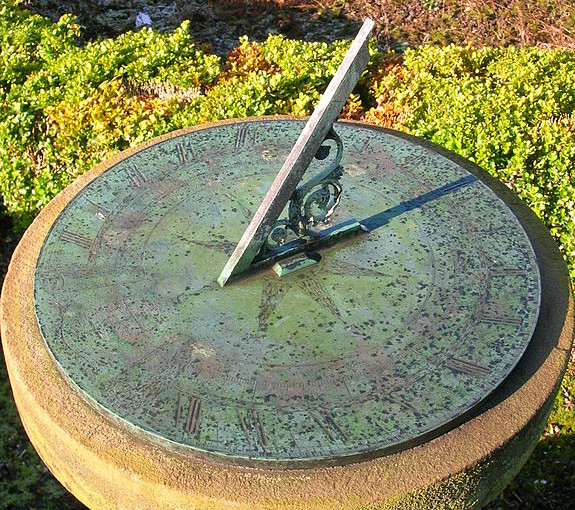
\includegraphics{sundial.jpg}
\end{image}
\begin{image}
  \begin{tikzpicture}
    \foreach \angle in { 270,280,...,450 }{
      \draw [ultra thick, yellow!70!orange, rotate around={\angle:(3,4)}]
      (3,3.5)--(3,3);
    };
    \draw[very thick, penColor,->] (0,0) -- (5,0);
    \draw[ultra thick,penColor4,->] (0,0) -- (3,2);
    \draw[ultra thick,penColor2,->] (0,0) -- (3,0);
    \draw[ultra thick, yellow!50!orange] (2.5,4)
    arc (180:360:.5);

    \draw[decoration={brace,mirror,raise=.2cm},decorate,thin] (0,0)--(3,0);
    \node at (1.5,-.5) {projection};

  \end{tikzpicture}
\end{image}



































\end{document}
